\chapter{Grafteori}
\usetikzlibrary{arrows, automata}

Dette kapitel har til formål at beskrive og redegøre for forskellige grafer og de vigtigste elementer i grafteori, og bygger på \citep{dmat} hvis ikke andet er angivet. 

Grafer kan bruges i mange tilfælde herunder kortlægning af veje i en by, kloaksystemer og forskellige kredsløb.
En simpel graf defineres formelt i Definition \ref{def_simpel_graf}.


\begin{defn}
En graf $G = (V, E)$ består af en mængde af knuder, $V$, og en mængde af kanter, $E$, hvor $V \neq \emptyset$.
Hver kant har enten en eller to knuder, den er forbundet til, og de beskrives som kantens endeknuder.
%En kant siges at forbinde dens endeknuder. Denne %konstruktion kaldes en \it{simpel graf}.
\label{def_simpel_graf}
\end{defn}

En kant repræsenteres ved en linje mellem to knuder, og knuder repræsenteres ved et punkt.
Har grafen enten et uendeligt antal knuder, kanter eller begge dele, er der tale om en \textit{uendelig graf}.
Ellers betegnes grafen som en \textit{endelig graf}.
I dette projekt vil der kun blive arbejdet med endelige grafer.

\begin{defn}
En graf kaldes \textit{simpel}, så længe der i grafen ikke findes to kanter, som forbinder samme knudepar, og enhver kant forbinder to forskellige knuder. 
Findes der i grafen to kanter, der forbinder samme knudepar, er der tale om en \textit{multigraf}, og forefindes der en eller flere kanter, der forbinder en knude til sig selv (en \textit{løkke}), er grafen en \textit{pseudograf}.
\end{defn}

\begin{figure}[h]
	\centering
	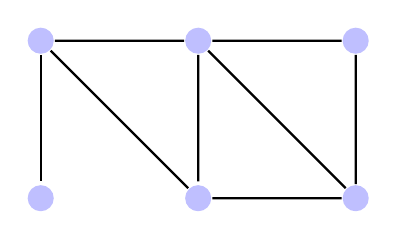
\begin{tikzpicture}[shorten >=1pt,auto,node distance=2cm,thick,main node/.style={circle,fill=blue!25}]                      
  \node[main node] (a) {};                                                                                                  
  \node[main node] (b) [left of=a] {};                                                                                      
  \node[main node] (c) [below of=a] {};                                                                                     
  \node[main node] (d) [left of=b] {};                                                                                      
  \node[main node] (e) [below of=b] {};                                                                                     
  \node[main node] (f) [below of=d] {};                                                                                     
                                                                                                                            
  \draw (c) -- (a) -- (b) -- (c) -- (e) -- (d) -- (b) -- (e);                                                               
  \draw (d) -- (f);                                                                                                         
\end{tikzpicture}

	\caption{Et eksempel på en simpel, endelig graf} \label{simpel_graf}
\end{figure}

I Figur \ref{simpel_graf} er der skitseret en simpel graf med seks knuder og otte forbindende kanter. Et eksempel på de multi- og pseudografer kan ses nedenfor i Figur \ref{Fig:Data1} og \ref{Fig:Data2}.

\begin{figure}[!htb]
   \begin{minipage}{0.48\textwidth}
     \centering
     \input{fig/tikz/multigraf}
     \caption{Et eksempel på en multigraf}\label{Fig:Data1}
   \end{minipage}\hfill
   \begin{minipage}{0.48\textwidth}
     \centering
     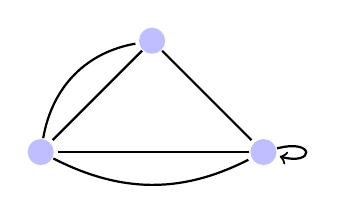
\begin{tikzpicture}[shorten >=1pt,auto,node distance=2cm,
                thick,main node/.style={circle,fill=blue!25}]

  \node[main node] (a) {};
  \node[main node] (b) [below left of=a] {};
  \node[main node] (c) [below right of=a] {};

  \path
    (a) edge node {} (b)
        edge node {} (c)
    (b) edge [bend left=35] node {} (a)
        edge [bend right=27] node {} (c)
    (c) edge [loop right] node {} (c)
        edge node [above] {} (b);
\end{tikzpicture}



     \caption{Et eksempel på en pseudograf}\label{Fig:Data2}
   \end{minipage}
\end{figure}

Det kan imidlertid være nødvendigt at give kanterne en retning for at indikere, i hvilken retning to knuder er forbundet.
I grafer, der eksempelvis repræsenterer trafikale netværk, kan det være nødvendigt at indikere, hvilken retning trafikken kører i eller at angive ensrettede strækninger.
Til disse formål vil en simpel graf være utilstrækkelig, idet kanterne deri netop ikke er retningsbestemte.

\begin{defn}
En orienteret graf $G = (V, E)$ består af en mængde knuder, $V$, og en mængde \textit{orienterede} kanter, $E$, hvor $V, E \neq \emptyset$.

En orienteret kant kan opfattes som et ordnet knudepar $(u,v)$ hvor $u,v \in  V$.
\label{def_retn_graf}
\end{defn} 

Definition \ref{def_retn_graf} tillader muligheden for, at et knudepar kan forbindes af op til flere orienterede kanter.
Findes dette i grafen, kaldes den en \textit{orienteret multigraf}, og denne må også indeholde løkker.
I det tilfælde, at alle knudepar kun forbindes af netop én orienteret kant, og der ingen løkker er, er grafen en \textit{simpel orienteret graf}.

\begin{figure}[h]
	\centering
	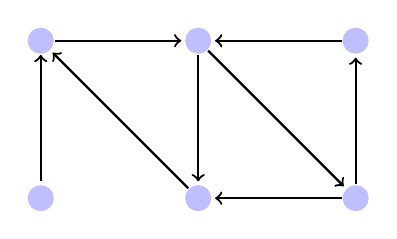
\begin{tikzpicture}[shorten >=1pt,auto,node distance=2cm,thick,main node/.style={circle,fill=blue!25}]                      
  \node[main node] (a) {};                                                                                                  
  \node[main node] (b) [left of=a] {};                                                                                      
  \node[main node] (c) [below of=a] {};                                                                                     
  \node[main node] (d) [left of=b] {};                                                                                      
  \node[main node] (e) [below of=b] {};                                                                                     
  \node[main node] (f) [below of=d] {};                                                                                     
                                                                                                                            
	\draw[->] (c) edge (a) (a) edge (b) (b) edge (c) (c) edge (e) (e) edge (d) (d) edge (b) (b) edge (e); 
	\draw[<-] (d) edge (f);                                                                                                         
\end{tikzpicture}

	\caption{Et eksempel på en orienteret graf, hvor pilene definerer retningen.}
\end{figure}

Eksempelvis er der i et netværk af computere brug for at kommunikation kan ske både frem og tilbage mellem enhederne.
Derfor er et simpelt orienteret system ikke tilstækkeligt.
Til dette kan der gøres brug af orienterede multigrafer.

\begin{figure}[h]
	\centering
	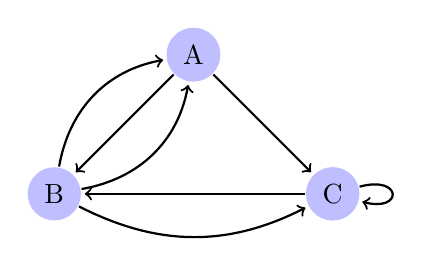
\begin{tikzpicture}[->,shorten >=1pt,auto,node distance=2.5cm,thick,main node/.style={circle,fill=blue!25}] 
  \node[main node] (a) {A};                   
  \node[main node] (b) [below left of=a] {B}; 
  \node[main node] (c) [below right of=a] {C};

  \path                                       
    (a) edge node {} (b)                      
        edge node {} (c)                      
    (b) edge [bend left=35] node {} (a)       
          edge [bend right=35] node {} (a)    
        edge [bend right=27] node {} (c)      
    (c) edge [loop right] node {} (c)         
        edge node [above] {} (b);             
    (a) edge [bend right=30] node {} (b)      
\end{tikzpicture}

	\caption{Et eksempel på en orienteret multigraf, hvor der både er adskillige kanter mellem knuderne A og B, samt er der en løkke tilstede i knudepunktet C.}
\end{figure}

Nogle gange er det nødvendigt at konstruere et netværk med både orienterede og ikke-orienterede kanter. Disse grafer kaldes \textit{kombinerede grafer}.

\begin{figure}[!h]
	\centering
	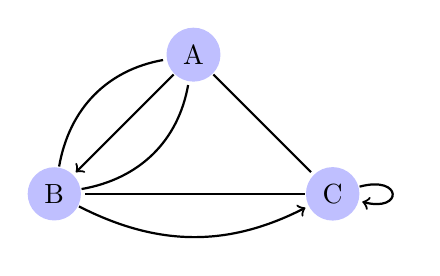
\begin{tikzpicture}[shorten >=1pt,auto,node distance=2.5cm,  
                thick,main node/.style={circle,fill=blue!25}]
                                                             
  \node[main node] (a) {A};                                  
  \node[main node] (b) [below left of=a] {B};                
  \node[main node] (c) [below right of=a] {C};               
                                                             
    \path [->] (a) edge node {} (b);                         
    \path      (a) edge node {} (c);                         
    \path      (b) edge [bend left=35] node {} (a);          
      \path      (b) edge [bend right=35] node {} (a);       
    \path [->] (b) edge [bend right=27] node {} (c);         
    \path      (c) edge [loop right] node {} (c);            
    \path      (c) edge node [above] {} (b);                 
\end{tikzpicture}

	\caption{Et eksempel på en kombineret graf hvor både orienterede og ikke-orienterede kanter indgår samt en løkke i knudepunktet C.}
\end{figure}

For at kunne danne et større overblik over de forskellige grafer, deres definition og karakteristika henvises der til Figur \ref{table:graf_oversigt}.

\begin{table}[h]
	\begin{tabular}{|c|c|c|c|}                                  
\hline                                                      
Type & Kanter & Flerdobbelte kanter tilladt & Løkker \\     
\hline                                                      
Simpel graf & Ikke-orienteret & Nej & Nej  \\               
                                                            
Multigraf & Ikke-orienteret & Ja & Nej \\                   
                                                            
Pseudograf & Ikke-orienteret & Ja & Ja \\                   
                                                            
Simpel orienteret graf & Orienteret & Nej & Nej \\          
                                                            
Orienteret multigraf & Orienteret & Ja & Ja \\              
                                                            
Kombineret graf & Orienteret og ikke-orienteret & Ja & Ja \\
\hline                                                      
\end{tabular}

	\caption{Et overblik over de forskellige graftyper} \label{table:graf_oversigt}
\end{table}

\usetikzlibrary{arrows, positioning}
\section{Grafterminologi}

Der findes begreber til at beskrive kanter og knuder i ikke-orienterede grafer, som bl.a. beskriver hvordan knuder og kanter er placeret i forhold til hinanden,, samt hvor mange knuder eller kanter, der er forbundet til en given knude.

\begin{defn}
To knuder, $u$ og $v$, siges at være naboer i en ikke-orienteret graf $G$, hvis $u$ og $v$ er endeknuder i en kant, $e$. Da betegnes $e$ som værende incident med både $u$ og $v$.
\end{defn}

\begin{defn}
En mængde af alle naboer til en knude, $v$, i en graf $G=(V,E)$ betegnes som $N(v)$, og kaldes et nabolag af $v$. Hvis $A$ $\subseteq$ $V$, betegner $N(A)$ mængden af alle knuder i $G$, som er nabo til mindst én knude i $A$.
\end{defn}

\begin{defn}
Graden af en knude, $v$, i en ikke-orienteret graf betegnes $\deg(v)$ og er antallet af kanter incidente med den givne knude.  En løkke vil bidrage med to til knudens grad. 
\end{defn}

En knude af nulte grad betegnes som værende \textit{isoleret} og har ingen incidente kanter. En knude af første grad betegnes som et \textit{vedhæng} og har netop én incident kant.

\begin{exmp}
Betragt grafen i Figur \ref{eksempel_nabo}. Graden af knuderne og nabolagene for knuderne kan her bestemmes. Samtidig kan isolerede knuder eller vedhæng identificeres.

Graden af en knude i grafen i Figur \ref{eksempel_nabo} bestemmes ved at identificere antallet af incidente kanter til knuden. Derfor er $\textrm{deg}(A)=1$, $\textrm{deg}(B)=3$, $\textrm{deg}(C)=3$, $\textrm{deg}(D)=4$, $\textrm{deg}(E)=3$ og $\textrm{deg}(F)=2$. 
Nabolagene for de enkelte knuder er mængden af naboknuder. 
Derfor er $N(A)=\lbrace B \rbrace$, $N(B)=\lbrace A, C, D \rbrace$, $N(C)=\lbrace B, D, E \rbrace$, $N(D)=\lbrace B, C, E, F \rbrace$, $N(E)=\lbrace C, D, F \rbrace$ og $N(F)=\lbrace D, E \rbrace$. 
I grafen er $A$ et vedhæng, og der forefindes ingen isolerede knuder.

\begin{figure}[h!]
	\centering
	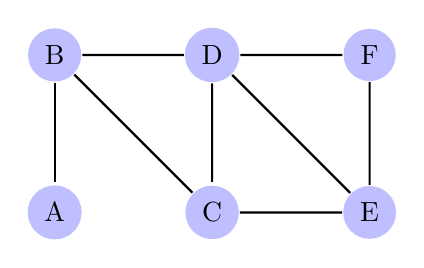
\begin{tikzpicture}[shorten >=1pt,auto,node distance=2cm,thick,main node/.style={circle,fill=blue!25}]                      
  \node[main node] (a) {F};                                                                                                  
  \node[main node] (b) [left of=a] {D};                                                                                      
  \node[main node] (c) [below of=a] {E};                                                                                     
  \node[main node] (d) [left of=b] {B};                                                                                      
  \node[main node] (e) [below of=b] {C};                                                                                     
  \node[main node] (f) [below of=d] {A};                                                                                     
                                                                                                                            
  \draw (c) -- (a) -- (b) -- (c) -- (e) -- (d) -- (b) -- (e);                                                               
  \draw (d) -- (f);                                                                                                         
\end{tikzpicture}

	\caption{En simpel ikke-orienteret graf} \label{eksempel_nabo}
\end{figure}
\end{exmp}

For at beskrive summen af graderne for alle knuder i en graf anvendes \textit{The Handshaking Theorem}. 

\begin{thm}\label{handshake}
	\textbf{The Handshaking Theorem}.
	Lad $G=(V,E)$ være en ikke-orienteret graf med $m$ kanter.
	Da er summen af knudernes grader
	\begin{align*}
		2m=\sum_{v \in V}\deg(v).
	\end{align*}
\end{thm}

\begin{proof}
	I en ikke-orienteret graf med $m$ kanter, bidrager hver kant i en graf med to grader - én grad til hvert endeknude.
	Det samlede antal grader for alle knuder i en graf stiger således med to per kant og summen af $\deg(v)$ er $2m$. 
\end{proof}

Som følge af Sætning \ref{handshake} er summen af knudernes grader et lige tal.

\begin{thm}
	En ikke-orienteret graf har et lige antal knuder af ulige grad.
\end{thm}

\begin{proof}
	Lad $V_1$ og $V_2$ være henholdsvis mængden af knuder af lige grad og mængden af knuder af ulige grad i en ikke-orienteret graf $G=(V,E)$ med $m$ kanter.
	Så er
	\begin{align*}
		2m=\sum_{v \in V}\deg(v)=\sum_{v \in V_1}\deg(v)+ \sum_{v \in V_2}\deg(v).
	\end{align*}
	Da $\deg(v)$ er lige for $v \in V_1$, er summen $\sum_{v \in V_1}\deg(v)$ også lige.
	Summen af de to led på højresiden i ligningen er lige, fordi de tilsammen er lig $2m$, og siden $\sum_{v \in V_1}\deg(v)$ er lige må det betyde at $\sum_{v \in V_2}\deg(v)$ også er lige.
	Summen $\sum_{v \in V_2}\deg(v)$ består af en række ulige tal, og for at summen bliver lige, skal der således være et lige antal ulige led i summen.
	Idet summen af graderne for knuderne af ulige grad i grafen er lige, må der være et lige antal af sådanne knuder.
\end{proof}

\section{Repræsentation af grafer}
Der er flere brugbare måder at repræsentere grafer på, og det ønskes at vælge den pæneste repræsentation. 
En overskuelig måde at repræsentere en graf på er ved matricer. 
To matricer, der almindeligvis bruges, er \textit{nabomatricer}, der er baseret på naboknuder, og \textit{incidensmatricer} baseret på incidensen af knuder og kanter. 

\begin{defn}
Lad $G=(V,E)$ være en simpel graf med $n$ knuder, hvor knuderne i $G$ står skrevet i vilkårlig rækkefølge som $v_1$, $v_2$, \dots , $v_n$.
Nabomatricen $A$ af $G$ er en $n \times n$ matrix, med 1 som den $(i,j)$’te indgang når $v_i$ og $v_j$ er naboer, og 0 er den $(i,j)$’te indgang, når de ikke er naboer. Hvis nabomatricen er $A=[a_{ij}]$, så er

\begin{align*}
	a_{ij}= \left\{\begin{array}{cc}
	1 & \textrm{hvis} \  \lbrace v_i, v_j \rbrace \  \in E \\
	0 & \textrm{ellers} .\\
	\end{array}\right.
\end{align*}
\end{defn}

En nabomatrice af en graf er baseret på den valgte ordning af knuderne, hvorfor der kan være $n!$ forskellige nabomatricer for en graf med $n$ knuder, idet der er $n!$ forskellige måder at ordne de $n$ knuder på.
Nabomatricen for en simpel ikke-orienteret graf er symmetrisk, hvilket betyder $a_{ij}=a_{ji}$, da begge indgange er 1, når de relaterede knuder er naboer, og 0 hvis de ikke er.
Da en simpel graf ikke indeholder løkker, er hver indgang $a_{ii}=0$ for alle $i=1,2,3, \dots ,n$. 

Nabomatricer kan også bruges til at repræsentere ikke-orienterede grafer med løkker og flere kanter til samme knude.
En løkke ved en knude $v_i$ er repræsenteret ved 1 ved position $(i,i)$ i nabomatricen.
Når flere kanter forbinder det samme par af knuder $v_i$ og $v_j$, eller der er flere løkker ved samme knude til stede, er nabomatricen ikke længere en nul-et matrice, idet den $(i,j)$’te indgang af matricen er lig antallet af kanter forbundet til $\lbrace v_i,v_j \rbrace$.
Alle ikke-orienterede grafer, herunder multi- og pseudografer, har symmetriske nabomatricer.

En anden almindelig måde at repræsentere grafer på, er ved incidensmatricer.

\begin{defn}
Lad $G=(V,E)$ være en ikke-orienteret graf med knuderne $v_1$, $v_2$, \dots , $v_n$ og kanterne $e_1$, $e_2$, \dots , $e_m$. Incidensmatricen, i forhold til ordningen af $V$ og $E$, er en $n \times m$ matrice, $M=[m_{ij}]$, hvor 

\begin{align*}
	m_{ij}= \left\{\begin{array}{cc}
	1 & \textrm{hvis} \  {e_j} \  \textrm{er} \  \textrm{incident} \ \textrm{med} \ v_i \\
	0 & \textrm{ellers}. \\
	\end{array}\right.
\end{align*}
\end{defn}

Incidensmatricer kan også bruges til at repræsentere flere kanter og løkker.
Flere kanter mellem samme to knuder er repræsenteret i incidensmatricen ved søjler med identiske indgange, idet disse kanter er incidente med det samme knudepar.
Løkker er repræsenteret ved en søjle med præcis én indgang lig 1, der svarer til den knude, der er incident med løkken.

\begin{exmp}
	For at illustrere eksempler på at opskrive en nabomatrice og en incidensmatrice, betragtes grafen i Figur \ref{fig:simple_graph_labels}. 
	
	\begin{figure}[h!]
		\centering
		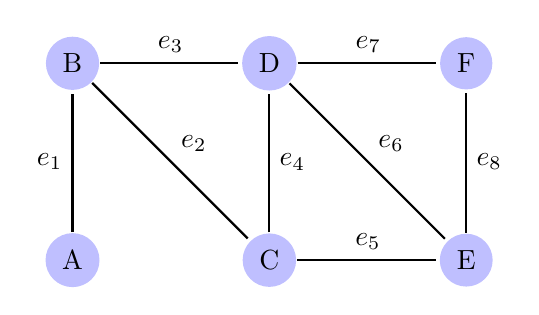
\begin{tikzpicture}[shorten >=1pt,auto,node distance=2.5cm,thick,main node/.style={circle,fill=blue!25}]                      
  \node[main node] (F) {F};                
  \node[main node] (D) [left of=F] {D};    
  \node[main node] (E) [below of=F] {E};   
  \node[main node] (B) [left of=D] {B};    
  \node[main node] (C) [below of=D] {C};   
  \node[main node] (A) [below of=B] {A};   
              
	\path[-, draw, thick]
  (A) edge node {$e_1$} (B)
	(B) edge node {$e_2$} (C)
	(B) edge node {$e_3$} (D)
	(C) edge node[right] {$e_4$} (D)
	(C) edge node {$e_5$} (E)
	(D) edge node {$e_6$} (E)
	(D) edge node {$e_7$} (F)
	(E) edge node[right] {$e_8$} (F)
	;
\end{tikzpicture}

		\caption{En simpel ikke-orienteret graf.} \label{fig:simple_graph_labels}
	\end{figure}
	
	Nabomatricen, $\mathbf{N}$, for grafen i Figur \ref{fig:simple_graph_labels} er en $6 \times 6$-matrice.
	Indgangen $n_{AA}=0$ angiver, at der ikke er er nogen løkker i $A$.
	Indgangen $n_{AB}=1$ angiver, at en kant forbinder $A$ og $B$, så $A$ og $B$ er naboer.
	På samme vis udfyldes resten af nabomatricen. 
	
	 \begin{equation*}
	  \mathbf{N}=
	  \begin{blockarray}{*{6}{c} l}
	    \begin{block}{*{6}{>{$\footnotesize}c<{$}} l}
	      A & B & C & D & E & F \\
	    \end{block}
	    \begin{block}{[*{6}{c}]>{$\footnotesize}l<{$}}
	      0 & 1 & 0 & 0 & 0 & 0 \bigstrut[t]& A \\
	      1 & 0 & 1 & 1 & 0 & 0 \bigstrut[t]&B \\
	      0 & 1 & 0 & 1 & 1 & 0 \bigstrut[t]&C \\
	      0 & 1 & 1 & 0 & 1 & 1 \bigstrut[t]& D \\
	      0 & 0 & 1 & 1 & 0 & 1 \bigstrut[t]& E \\
	      0 & 0 & 0 & 1 & 1 & 0 \bigstrut[t]& F \\
	    \end{block}
	  \end{blockarray}
	\end{equation*} 
	
	Incidentmatricen, $\mathbf{M}$, for grafen i Figur \ref{fig:simple_graph_labels} er en $6 \times 8$-matrice.
	Indgangen $m_{A,e_1}=1$ angiver, at $e_1$ er incident med $A$.
	Indgangen $m_{A,e_2}=0$ angiver, at $e_2$ ikke er incident med $A$ og så videre.
	
	 \begin{equation*}
	  \mathbf{M}=
	  \begin{blockarray}{*{8}{c} l}
	    \begin{block}{*{8}{>{$\footnotesize}c<{$}} l}
	      $e_1$ & $e_2$ & $e_3$ & $e_4$ & $e_5$ & $e_6$ & $e_7$ & $e_8$ \\
	    \end{block}
	    \begin{block}{[*{8}{c}]>{$\footnotesize}l<{$}}
	      1 & 0 & 0 & 0 & 0 & 0 & 0 & 0 \bigstrut[t]& A \\
	      1 & 1 & 1 & 0 & 0 & 0 & 0 & 0 \bigstrut[t]&B \\
	      0 & 1 & 0 & 1 & 1 & 0 & 0 & 0 \bigstrut[t]&C \\
	     0 & 0 & 1 & 1 & 0 & 1 & 1 & 0 \bigstrut[t]& D \\
	      0 & 0 & 0 & 0 & 1 & 1 & 0 & 1 \bigstrut[t]& E \\
	     0 & 0 & 0 & 0 & 0 & 0 & 1 & 1 \bigstrut[t]& F \\
	    \end{block}
	  \end{blockarray}
	\end{equation*}
\end{exmp} 

\section{Komplette grafer}
En komplet graf er en graf hvor et hvert unikt par af knuder i grafen er forbundet.
En komplet graf navngives $K_n$ hvor $n$ er antallet af knuderf i grafen.
I figur \ref{fig:komplette_grafer} ses de første 5 komplette grafer.
En graf hvor mindst ét par af knuder ikke er forbundet, kaldes en ikke-komplet graf.

\begin{figure}[h]
	\centering
	% Radius of regular polygons
\newdimen\R
\R=1cm

\begin{tikzpicture}
  \foreach \x in {1,2,3,4,5}{
    \node[yshift=-1.5\R, xshift=\x*2.5\R-2.5\R] {$K_\x $};
  }
  \begin{scope}[every node/.style={circle,fill=blue!25}]
    \node (0:0);

    \foreach \x in {1,2}{
      \node[xshift=2.5\R] (\x) at (\x*180-180:\R);
    }
    \path (1) edge (2);

    \foreach \x in {1,2,3}{
      \node[xshift=5\R] (\x) at (\x*120-120:\R);
    }
    \path (1) edge (2);
    \path (2) edge (3);
    \path (3) edge (1);
  
    \foreach \x in {1,2,3,4}{
      \node[xshift=7.5\R] (\x) at (\x*90-90:\R);
    }
    \foreach \x in {1,2,3}{
      \path (4) edge (\x);
    }
    \foreach \x in {1,2}{
      \path (3) edge (\x);
    }
    \path (1) edge (2);
  
    \foreach \x in {1,2,3,4,5}{
      \node[xshift=10\R] (\x) at (\x*72-72:\R);
    }
    \foreach \x in {1,2,3,4}{
      \path (5) edge (\x);
    }
    \foreach \x in {1,2,3}{
      \path (4) edge (\x);
    }
    \foreach \x in {1,2}{
      \path (3) edge (\x);
    }
    \path (1) edge (2);
  \end{scope}
\end{tikzpicture}

	\caption{De første $5$ komplette grafer} \label{fig:komplette_grafer}
\end{figure}

Antallet af kanter i en komplet graf $K_n$ afhænger kun af $n$.

\begin{thm}
	For en komplet graf $K_n = (V_n, E_n)$ med $n$ knuder er $|E_n|$ antallet af kanter. Da er
	\begin{align*}
		|E_n| = \frac{n (n - 1)}{2}
	\end{align*}
\end{thm}
\begin{proof}
	For at gennemføre et induktionsbevis skal basisskridtet og induktionsskridtet gennemføres.
	Lad propositionen $P(n)$ være at $|E_n|= \frac{n (n - 1)}{2}$, hvor $n$ er antal knuder i en komplet graf $K_n$ og $m$ være antal kanter.

	\textit{Basisskridt:} $K_1$ består af en enkelt knude, og da der ikke er et par af knuder i grafen, må der da ikke eksistere nogen kanter.
	$\frac{ 1 \cdot 0}{2} = 0$, hvilket betyder at $P(1)$ er sand. Da er basisskidtet gennemført.

	\textit{Induktionsskridt:} Det skal nu vises at der for et vilkårligt $k$ gælder at $P(k) \to P(k + 1)$, altså at $|E_k| = \frac{k (k - 1)}{2}$ medfører at $|E_{k+1}| = \frac{k (k + 1)}{2}$.

	Antag at $|E_k| = \frac{k (k - 1)}{2}$ for $K_k$.
	Den næste komplette graf $K_{k+1}$ må være den graf hvor der er én til knude. Denne nye knude $v$ skal være forbundet til alle knuder i $K_k$ for at være en komplet graf. $\deg (v)$ må da være lig $k$. Da må
	\begin{align*}
		|E_{k+1}| 
		= |E_k| + k
		= \frac{k (k - 1)}{2} + k
		= \frac{k^2 - k}{2} + \frac{2k}{2}
		= \frac{k^2 + k}{2} 
		= \frac{k (k + 1)}{2}
	\end{align*}
	Dette er netop $P(k + 1)$, hvilket betyder at induktionsskridtet er gennemført.
\end{proof}

% \section{Parring i grafer}
Nogle grafer har den egenskab, at deres knuder kan deles op i to undergrupper, således at knuder fra den samme undergruppe ikke forbindes af kanter, men kun forbindes med knuder fra den anden undergruppe.
Dette kaldes parring i grafer.

Parring i grafer kan blandt andet bruges til at vise relationer mellem to forskellige typer objekter.
Et eksempel på dette kan være en graf, der viser hvilke studerende der tager hvilke kurser, så de studerende er i en undergruppe og kurserne i en anden. 

\begin{defn}
	En simpel graf $G$ kaldes parret, hvis dens knuder kan deles op i to adskilte undergrupper, $V_1$ og $V_2$, hvor $V_1 \cap V_2 = \emptyset$, så enhver kant i grafen forbinder en knude fra $V_1$ og $V_2$, men ikke to knuder fra den samme undergruppe.
	Når dette gælder, kaldes parret ($V_1,V_2$) en parring af $V$ i $G$.
\end{defn}

\begin{exmp}
	I Figur \ref{parret_graf} ses en parret graf, med de to undergrupper ($v_1,v_2,v_3$) og ($v_4,v_5$). 
	På grafen ses det, at hver kant forbinder en knude fra den ene undergruppe med en fra den anden, mens ingen kanter forbinder to knuder fra den samme undergruppe. 
	Deruder ses det også, at der ikke er en kant fra alle knuder i en gruppe til alle knuder i den anden gruppe.
	Der er for eksempel ikke en kant mellem $v_3$ og $v_5$. 
	Der behøver ikke være kanter fra alle knuder i den ene undergruppe til den anden for at grafen er parret.
	Havde der været en kant mellem $v_1$ og $v_2$ havde grafen ikke været parret, da der ikke må være en kant mellem to knuder fra samme undergruppe.
\end{exmp}

\begin{figure}[h]
	\centering
	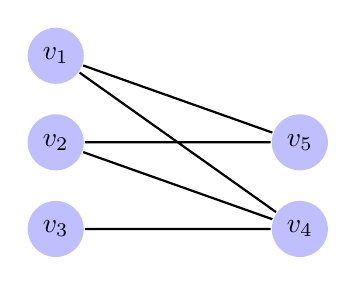
\begin{tikzpicture}[auto, thick, node distance=1.1cm,every node/.style={circle,fill=blue!25}]
	\node (p0) {$v_1$};
	\node (p1) [below of=p0] {$v_2$};
	\node (p2) [below of=p1] {$v_3$};
	\node (p3) [right of=p2,xshift=2cm] {$v_4$};
	\node (p4) [above of=p3] {$v_5$};
	
	\draw
	(p0) -- (p3)
	(p0) -- (p4)
	(p1) -- (p3)
	(p1) -- (p4)
	(p2) -- (p3);
\end{tikzpicture}

	\caption{Et eksempel på en parret graf} \label{parret_graf}
\end{figure}

\begin{thm}
	En simpel graf er parret hvis og kun hvis, det er mulig at tildele hver knude en af to farver, således at hver kant ikke forbinder to knuder af samme farve. 
\label{farve_satning}
\end{thm}

\begin{proof}
	Antag at $G=(V,E)$ er en parret simpel graf. Så er $V=V_1 \cup V_2$, hvor $V_1 \cap V_2 = \emptyset$ og hver kant i $E$ forbinder en knude i $V_1$ med en knude i $V_2$. 
	Tildeles en farve til alle knuder i $V_1$ og en anden farve til alle knuderne i $V_2$, så vil ingen kanter forbinde to knuder af samme farve. 

	Antag nu, at det er muligt at tildele farver til knuder, hvor der kun bruges to farver, hvor hvert knudepar består af to knuder af hver sin farve.
	Da må $V_1 \cap V_2= \emptyset$ og $V=V_1 \cup V_2$.
	Ydermere forbinder hver kant en knude i $V_1$ til en knude i $V_2$, da ingen naboknuder kan tilhøre samme undergruppe. 
\end{proof}

\begin{exmp}
	I Figur \ref{farve_graf} ses en parret graf, hvor hver knude er tildelt en farve jævnfør sætning \ref{farve_satning}. 
	Her ses det, hvordan hver kant forbinder en rød knude med en blå knude, samt hvordan ingen kant forbinder to røde eller to blå knuder.
	
	\begin{figure}[h!]
		\centering
		 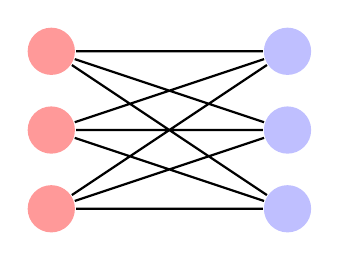
\begin{tikzpicture}[auto,thick,every node/.style={circle, minimum size=0.6cm,fill=blue!25}]
 	\node (p0) [fill=red!40]{};
 	\node (p1) [below of=p0, fill=red!40] {};
 	\node (p2) [below of=p1, fill=red!40] {};
 	\node (p3) [right of=p2,xshift=2cm] {};
 	\node (p4) [above of=p3] {};
 	\node (p5) [above of=p4] {};

 	\draw       
 	(p0) -- (p3)
 	(p0) -- (p4)
 	(p1) -- (p3)
 	(p1) -- (p4)
 	(p2) -- (p3)
 	(p2) -- (p4)
 	(p5) -- (p0)
 	(p5) -- (p1) 
 	(p5) -- (p2);    
 \end{tikzpicture}                

		\caption{En farveopdelt parret graf}\label{farve_graf}
	\end{figure}
\end{exmp}

En parring kan også være komplet. 
At en parring er komplet betyder, at hver knude fra en undergruppe er forbundet med alle knuder fra den anden undergruppe. 
En sådan graf betegnes $K_{m,n}$, hvor $m$ er antallet af knuder i den ene undergruppe og $n$ antallet i den anden undergruppe. 

\begin{exmp}
	Grafen i Figur \ref{farve_graf} er også en komplet parring, fordi hver rød knude er forbundet med hver blå knude. 
Denne graf kaldes derfor $K_{3,3}$
\end{exmp}

